\chapter{GLOBALLY SPATIAL-TEMPORAL PERCEPTION: A LONG-TERM TRACKING SYSTEM}\label{chap:globally}

\section{Abstract}
Although siamese trackers have achieved superior performance, these kinds of approaches tend to favour the local search mechanism and are thus prone to accumulating inaccuracies of predicted positions, leading to tracking drift over time, especially in long-term tracking scenario. To solve these problems, we propose a siamese tracker in the spirit of the faster RCNN's two-stage detection paradigm. This new tracker is dedicated to reducing cumulative inaccuracies and improving robustness based on a global perception mechanism, which allows the target to be retrieved in time spatially over the whole image plane. Since the very deep network can be enabled for feature learning in this two-stage tracking framework, the power of discrimination is guaranteed. What's more, we also add a CNN-based trajectory prediction module exploiting the target's temporal motion information to mitigate the interference of distractors.
These two spatial and temporal modules exploit both the high-level appearance information and complementary trajectory information to improve the tracking robustness. Comprehensive experiments demonstrate that the proposed Globally Spatial-Temporal Perception-based tracking system performs favorably against state-of-the-art trackers.

\section{Introduction}
\label{sec:intro}

Object tracking \cite{Leang2018OnlineFO, Wang2019VisualOT, Zhang2018UsingFL} is a challenging problem in the field of computer vision, which aims to establish the positional relationship of the object to be tracked in a continuous video sequence.
The popular siamese trackers \cite{SiamFC, SiamRPN, Wang2018SiamMask} are typically based on the local search mechanism: \HL{searching the target} within a small neighborhood centered on the target position of the previous frame to determine \HL{its current position}.
This mechanism works \HL{well if} the target only has a small displacement between two adjacent frames.
\HL{It also brings benefits in another aspect, which is} to avoid interference from the distractors in the background.

\begin{figure}[t]
    \centering
    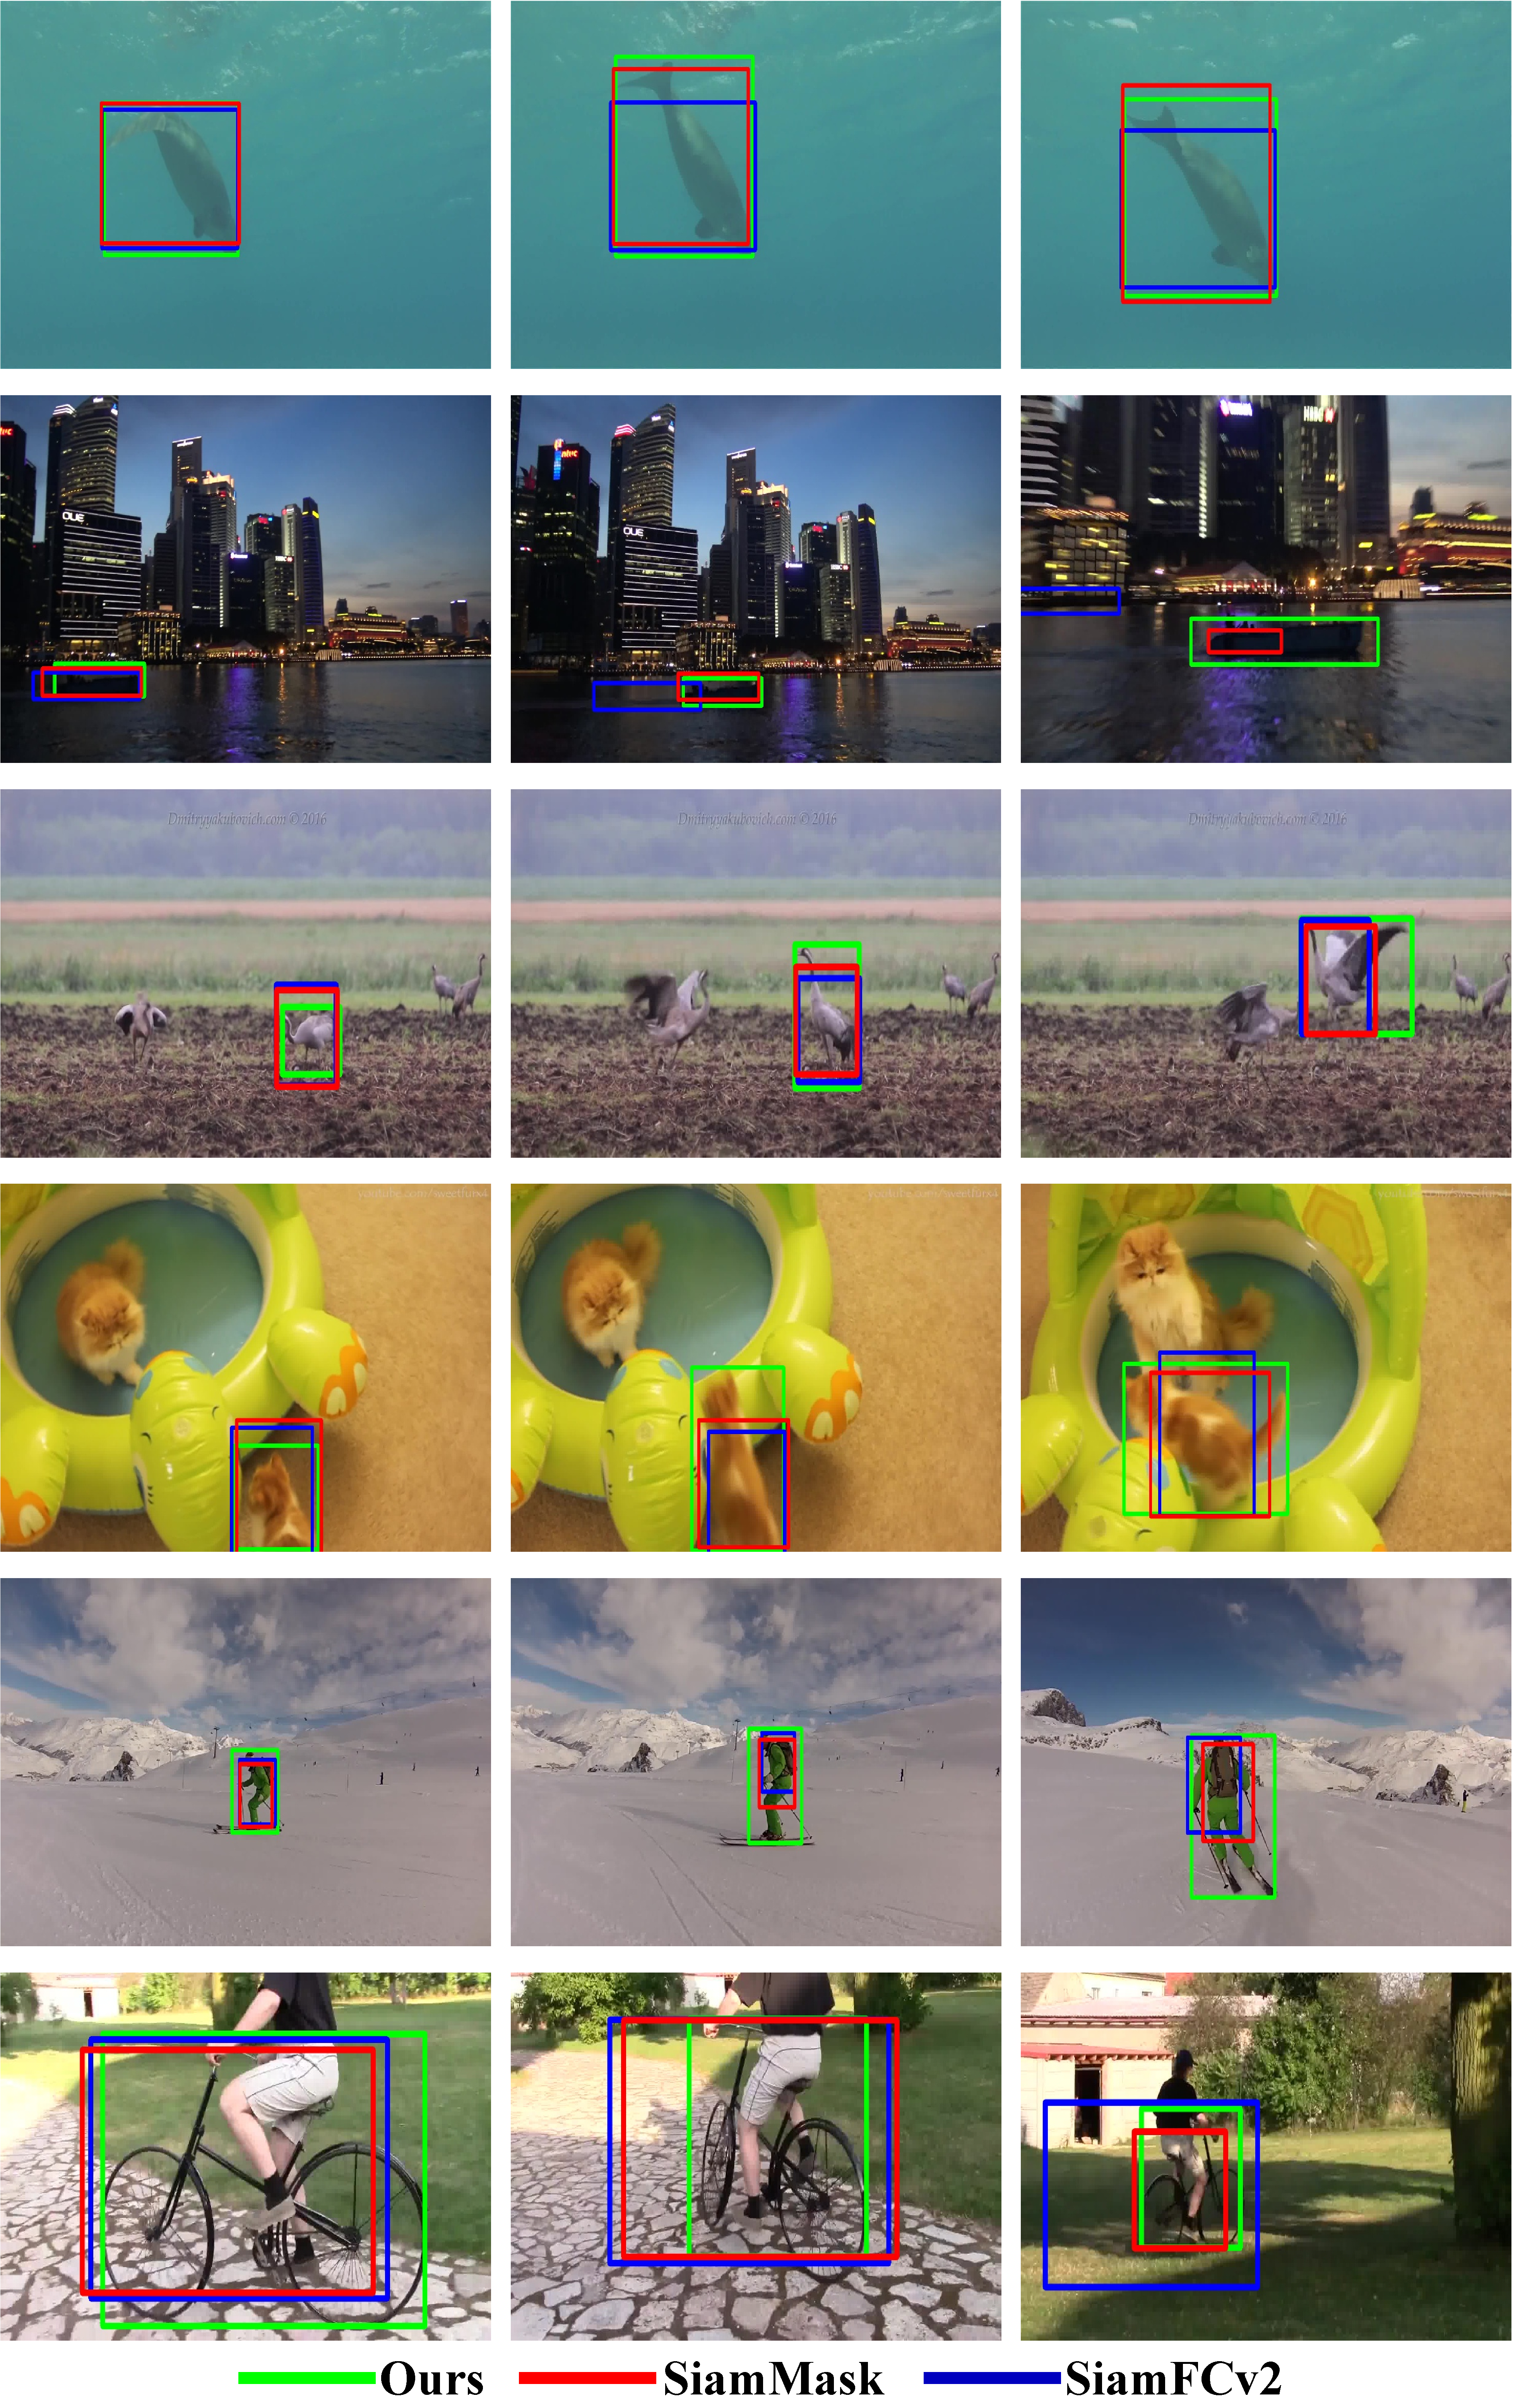
\includegraphics[width=1.0\textwidth]{Img/globally/visulization.pdf}
    \caption{A comparison of our method with the stage-of-the-art trackers SiamMask \cite{Wang2018SiamMask} and SiamFCv2 \cite{SiamFC} in challenging situations. The example frames are from the GOT-10k \cite{GOT-10k} testing set.
    % Our approach performs better compared to existing approaches.
    }
    \label{fig:visulization}
\end{figure}

However, the local search mechanism \HL{bears} some shortcomings.
First, \HL{it could cause irreversible cumulative errors if the predictions of the target positions in the previous frames drift away due to challenging illumination change, motion blur, \textit{etc.}, because the search area generated in the current frame may not cover the target leading to a complete failure in subsequent frames.}
\HL{Second, it is difficult for the local mechanism-based trackers} to meet the needs of long-term tracking \cite{kalal2011tracking, hong2015multi}.
Under the long-term \HL{scenario, the target frequently re-enters and re-exits} the screen.
\HL{Since the tracker cannot set the correct search area when the target leaves and re-enters the screen, it often fails to retrieve the target due to the wrong search area without the target covered.}

Inspired by faster RCNN's two stage detection paradigm \cite{ren2015faster}, we propose a \HL{siamese} tracker based on the global perception mechanism.
During the tracking process, \HL{our tracker} is always able to perceive the target \HL{over} the entire image.
Therefore, even if the tracker makes a mistake due to \HL{the challenging target appearance variations, the target can still be retrieved in time once its appearance returns to normal. Especially under the long-term out-of-view disappearance scenario, where the tracker cannot find the target in the full image when the target leaves the screen, our tracker can continue to work when the target re-enters the screen from any position.}

\HL{Besides the above globally spatial perception mechanism, we also propose a temporal motion model to mitigate the interference of distractors. It is known that the siamese-based tracking framework is sometimes plagued by distractors because it is difficult for the end-to-end trained siamese matching network to distinguish well between objects that look very similar. Different from the simply designed hand-crafted strategies \cite{SiamFC, SiamRPN}, our proposed CNN-based motion model is end-to-end trained and can predict the target current position distribution using its historical trajectory information and current target appearance information.}
\HL{Specifically,} the motion \HL{patterns} are automatically learned from the trajectory dataset \HL{in the training phase instead of} the hand-crafted features or rules \cite{iswanto2017visual}\HL{; in the testing phase,} we can use the position information of any number of historical frames instead of just the previous frame for prediction.

\iffalse
Another advantage of this globally spatial-temporal perception mechanism is that it use the RoI Align \cite{He2018MaskR} operation to enable the tracker to take advantage of deeper networks \HL{for feature learning, which is not acceptable for the popular local mechanism-based SiamFC \cite{SiamFC} and SiamRPN \cite{SiamRPN} trackers, because the padding in their network structures} will destroy the strict translation invariance \cite{SiamFC}. \HL{Specifically}, the entire template image and search image in our tracker are sent to the same backbone network to extract features,  \HL{and} then the object features are obtained \HL{using} the RoI Align operation from the template features according to the ground truth of the \HL{initial frame}. The object features and the search \HL{image} features are cross-correlated by channel to obtain \HL{a fusion feature map}, which \HL{is} sent to the subsequent tracking \HL{modules}. \HL{Since this new} solution has no restrictions on the \HL{translation invariance, we} can use the powerful ResNet \cite{he2016deep} as the backbone network \HL{to accurately model the discrimination between the foreground object and background clutters.}
\fi

\iffalse
To sum up, this paper makes following three main contributions.
(1) Based on the global perception mechanism, we introduce a two stage tracking pipeline using a very deep network to reduce cumulative inaccuracies and improve robustness.
(2) A novel unified end-to-end convolutional neural network architecture \HL{for} trajectory prediction is proposed, where historical trajectory information and appearance information of the current frame are used to predict the target position distribution.
(3) We demonstrate the effectiveness of our proposed 
Globally Spatial-Temporal Perception-based tracking system (GSTP)
\HL{by showing} that the tracking performance \HL{performs favorably against}
other state-of-the-art approaches on the \HL{GOT-10k \cite{GOT-10k} and UAV20L \cite{mueller2016benchmark} Long-term Tracking datasets}.
\fi

\section{THE PROPOSED ALGORITHM}
\label{sec:method}

\iffalse
\begin{figure}[t]
    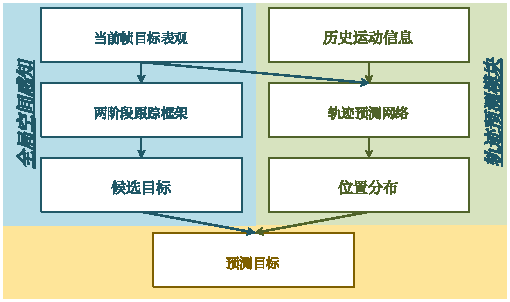
\includegraphics{images/Arch7.pdf}
    \caption{Architecture of our Globally Spatial-Temporal Perception-based (GSTP) tracking system.}
    \label{fig:arch}
\end{figure}
\fi

\iffalse
\begin{figure*}
    \centering
    \includegraphics[width=12cm]{images/NetworkStructure1.pdf}
    \caption{The proposed tracking framework.}
    \label{fig:network}
\end{figure*}
\fi

\iffalse
\begin{figure*}
    \centering
    \includegraphics[width=12cm]{images/MotionModel.pdf}
    \caption{The effect of the motion model. SiamRCNN detects the real target (in green box) and the distractor (in red box). The motion model predicts the position distribution measuring the likelihood that the target is located at each spatial location. The motion model eliminates the distractor and preserves the real target.}
    \label{fig:motion_model}
\end{figure*}
\fi

Our method explores the key idea that the task of visual object tracking can be tackled by splitting it into first extracting candidate targets, followed by eliminating distractors using the motion model.
By adopting this paradigm, we can achieve better performance by designing a more accurate tracking component and a more robust motion model, especially in the long-term scenario.

%To solve the cumulative error caused by local search, 
Specifically, we propose the Globally Spatial-Temporal Perception tracking system, which means: (1) We use an entire image instead of a small image patch as the input to the tracker to provide the global spatial information for it.  (2) In order to better perceive the global spatial information, we propose a two-stage tracking component, which is able to detect candidate targets that are visually similar to the ground truth target. (3) To perceive the temporal information, we propose a motion model, which is able to exclude the distractors by predicting the location distribution to obtain the final tracking result.

\iffalse
Most state-of-the-art trackers adopt a one-stage framework, which performs classification and bounding box regression only once based on features obtained by cross-correlation.
In the field of object detection, the performance of two-stage detectors is usually better than that of one-stage detectors.
Inspired by this, we design our tracker as a two-stage network.
The RPN stage rapidly filters out most background samples, and the RoI head adopts a fixed foreground-to-background ratio to maintain a manageable balance between foreground and background.
In addition, two steps of regressions achieve accurate localization even for objects with extreme shapes.
\fi

\subsection{Tracking component}

We build our tracking component based on the popular object detection architecture --- faster RCNN \cite{ren2015faster}. Although the use of object detection modules and siamese-based feature extractor for object tracking is not first proposed in this paper, our tracker has advantages over relevant tracking algorithms \cite{SiamRPN, Wang2018SiamMask, danelljan2019atom, voigtlaender2019siam}. Compared with SiamRPN \cite{SiamRPN}, whose input is always image patches with target located at the center, the input of our tracking component is the entire image, which means the target may appear at any spatial location. This prevents the network from learning bias to the center location, thereby breaking the spatial invariance restriction \cite{SiamRPN++} of the network architecture. As a result, the very deep networks such as ResNet50 \cite{he2016deep} can be used as the feature extractor of the tracking component. For detailed explain about spatial invariance restriction and center bias, please refer to \cite{SiamRPN++}.
%because the input of the network is the entire image, instead of the image patch centered on the target, the target will appear in any poisition in the image, so we do not need the network has strict spatial invariance restriction \cite{SiamRPN++}, so we can use a deeper feature extractor, i.e., resnet50. 
Compared with SiamRPN \cite{SiamRPN} and SiamMask \cite{Wang2018SiamMask}, we use a two stage architecture. The second stage (RoI head \cite{ren2015faster}) can distinguish the foreground and background more effectively.
Compared with SiamMask \cite{Wang2018SiamMask} and ATOM \cite{danelljan2019atom}, our tracker can search for the target in the whole image, which allows the target to be retrieved in time spatially after the tracking module makes a mistake.
Compared with Siam R-CNN \cite{voigtlaender2019siam}, whose backbone and RPN are frozen, our tracker generate the target-specific features before RPN, and the whole network can be trained end to end. In object tracking, a target may be foreground in one video and background in another. Therefore, the candidates generated by our RPN can better meet the requirements of general object tracking.
%(The backbone and RPN are frozen and only the redetection head (after concatenation) is trained for tracking) they fixed the parameters in the backbone and the RPN. Only the second stage is used for target spercific tracking, which is not good for "generatic" object tracking: because some objects are foreground in some cases and background in others. Instead, our tracker use the correlation before RPN, the "target" which is good for general object tracking. The architecture of our tracking component is described as follows:

%The first component of our tracking framework (i.e., SiamRCNN) is a two-stage tracker (Fig. \ref{fig:siamrcnn}) used to detect object regions that are visually similar to the given first-frame template object.
%Specifically, the tracking component consists of four modules: (1) feature extraction module, (2) feature fusion module, (3) RPN head module, and (4) RoI head module.

%The transplant from a detection task to a tracking task using faster RCNN is straightforward and easy to implement.
%, which is another advantage of our tracking module. 
To describe our tracking component, we we first briefly revisit faster RCNN. It consists of a feature extractor followed by two detection stages: the RPN head and the RoI head.
The feature extractor $\phi_{1}$ is a variant of ResNet50. The first stage uses a region proposal network (RPN) to slide on the last feature map of the backbone layers and predict whether there is an object or not and also predict the bounding box of those objects. The second stage (\textit{i.e.}, RoI head) is run for each region proposed by the RPN by performing RoI Align \cite{He2018MaskR} to extract deep features from this proposed region. 
Each RoI (Region of Interest) is classified as a specific category using a classification layer and the bounding box is refined using a regression layer.
Please refer to \cite{ren2015faster} for more detailed information.

For the task of object tracking, there are two inputs to the feature extractor $\phi_{1}$: the template image $z$ and the search image $x$. According to the design of the siamese architecture, the two inputs share the same network parameters to extract features.
After generating the template feature $f_{z} = \phi_{1}(z)$ and search feature $f_{x} = \phi_{1}(x)$, we crop the object feature $f_{obj} \in \mathbb{R}^{1024 \times 7 \times 7}$ by the RoI Align operation \cite{He2018MaskR} from the template features according to the ground truth of the target:
\begin{equation}
    f_{obj} = \mathcal{R}(b_{obj}, f_{z}),
\end{equation}
where $\mathcal{R}$ represents the RoI Align operator and $b_{obj}$ is the ground truth bounding box of the target.
Next, the search feature and the object feature are merged via the depth-wise cross-correlation \cite{SiamRPN++}:
\begin{equation}
    f_{corr} = f_{obj} * f_{x},
\end{equation}
where $f_{corr}$ is the fusion feature and $*$ is the depth-wise cross-correlation operator.
%The use of RPN (region proposal network) is ...
Then $f_{corr}$ is sent to the RPN head to generate candidates $B=\{b^{i}_{roi}\}^{i=1:N}$.
\iffalse
There are two inputs to the feature extraction module: the template image $z$ and the search image $x$. According to the design of the siamese architecture, the two inputs share the same network parameters to extract features.
The network structure of the feature extraction module is a variant of ResNet50, which is pretrained on the 1000-class ImageNet classification set. Features of the input images are extracted from the final convolution layer of the 4-th stage. The obtained template features $f_{z} = \phi(z)$ and search features $f_{x} = \phi(x)$ with channel dimension 1024 and stride 16 are sent to the subsequent feature fusion module.

In the feature fusion module, object features $f_{obj}$ are obtained by the RoI Align operation from the template features according to the ground truth of the target. The search features and the object features are merged via the depth-wise cross-correlation:
\begin{equation}
    f_{obj} = \mathcal{R}(b_{obj}, f_{z})
\end{equation}
where $\mathcal{R}$ represents the RoIAlign, $\odot$ represents the element-wise multiplication, $b$ represents an RoI in candidate proposals and $\mathcal{X}$ represents the fused feature of $b$.
\begin{equation}
    f_{corr} = f_{obj} * f_{x}.
\end{equation}
Two 1 $\times$ 1 convolutions with channel dimension 1024 are added on top of the correlation layer to obtain the fusion feature.

The RPN head includes two sibling 1 $\times$ 1 convolutional layers -- a classification layer with channel dimension 2$k$, and a regression layer with channel dimension 4$k$, where $k$ is the number of maximum possible proposals for each location. The RPN head takes the fusion feature as input and simultaneously regress region bounds and objectness scores for each anchor.
\fi
%The RoI head is run for each region proposed by the RPN by performing RoI Align \cite{He2018MaskR} to extract deep features from this proposed region.
At a second stage, the RoI Align operation is performed on the fusion feature $f_{corr}$, generating a small feature map with a channel dimension of 2048 and a fixed spatial extent of 7 $\times$ 7 for every RoI:
\begin{equation}
    f_{roi}^{i} = \mathcal{R}(b_{roi}^{i}, f_{corr}),
\end{equation}
where $b_{roi}^{i}$ is the bounding box of candidate region $i$.
Finally, each RoI is classified as foreground/background. During testing, we select top $K$ ranked RoI as the candidate targets, which will be post-processed in the motion model.

\iffalse
The RoI Aligned features are fed into the global average pooling layer followed by two sibling output layers: one that produces softmax probability estimates over two classes (foreground or background) and another layer that outputs four real-valued numbers for the foreground class. These four values encode the refined bounding-box position for the RoI.
The loss of SiamRCNN is:
$$Loss = L_{cls}^{rpn} + L_{cls}^{roi} + \lambda (L_{reg}^{rpn}+L_{reg}^{roi}),$$
where $\lambda$ is hyper-parameter to balance the classification loss and the regression loss. $L_{cls}^{*}$
is the cross entropy loss and $L_{reg}^{*}$ is the standard smooth $L1$ loss for regression.
\fi

\iffalse
\begin{figure*}
    \centering
    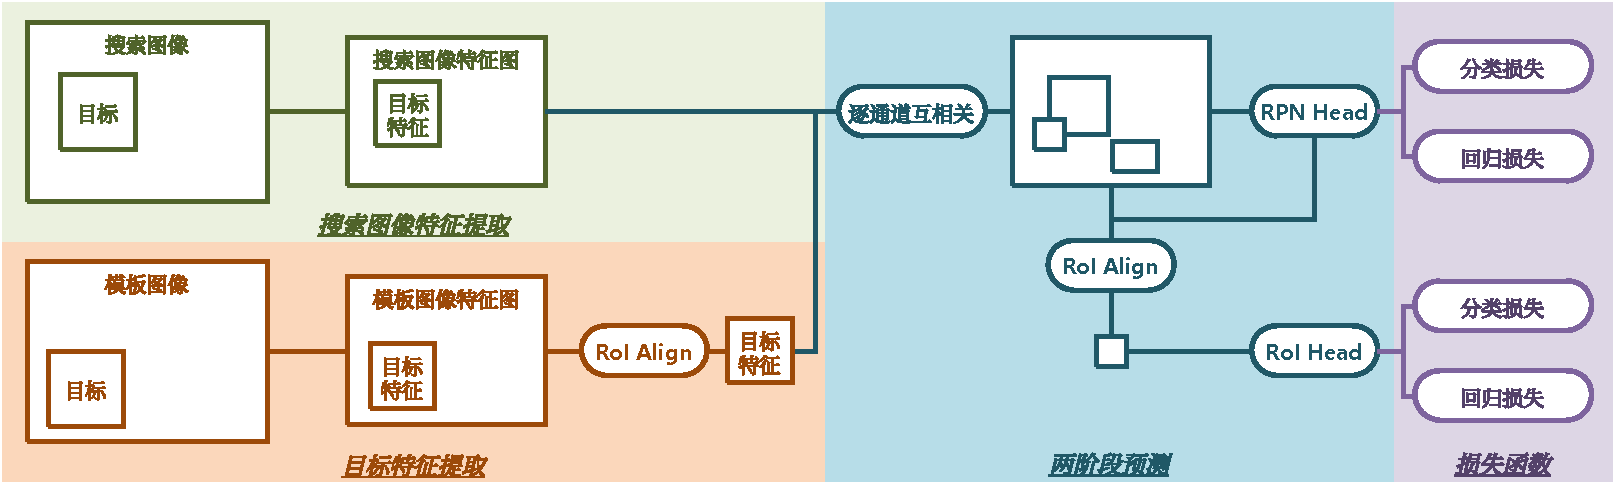
\includegraphics[width=17cm]{images/SiamRCNN.pdf}
    \caption{Architecture of SiamRCNN.}
    \label{fig:siamrcnn}
\end{figure*}
\fi

\subsection{Motion model} After detecting object regions that are visually similar to the given first-frame template object with our tracking component, we use a motion model to eliminate distractors and obtain the final tracking result.
The motion model works in an end-to-end manner by learning the target position distribution using historical trajectory information and appearance information of the current frame.
It then rescores the candidate targets according to the position distribution, which is a 2D heatmap measuring the likelihood that the target is located at each spatial location.

Let $H_{t}^{k} = \{h_{t-i}\}_{i=1:k}$ denote the historical trajectory information, where $t$ is the index of the current frame, $k$ is the length of history, and $h_{j} = \{x_{j}, y_{j}\}$ is a two-dimensional coordinate representing the position of the target in frame $j$.
Inspired by the pose estimation task, we present $h_{j}$ as a two-dimensional heatmap $m_{j} \in \mathbb R^{h \times w}$ with a 2D Gaussian centered on the target position $(x_{j}, y_{j})$.
To model the temporal information,  The generated $k$ heatmaps are concatenated according to the time order to obtain the trajectory tensor $\mathcal{M} \in \mathbb{R}^{k \times h \times w}$ with channel dimension $k$: 
\begin{equation}
    \mathcal{M}_{t}^{k} = \mathcal{C}(m_{t-k}, m_{t-k+1}, ..., m_{t-1}),
\end{equation}
where $\mathcal{C}(\cdot)$ is the concatenation operation.

Our motion model not only utilizes the historical trajectory information for prediction, but also considers the appearance information of the current frame.
To achieve this, the RGB image of the current frame $\mathcal{I} \in \mathbb{R}^{3 \times h \times w}$ and the trajectory tensor are concatenated to obtain the enhanced trajectory tensor $\mathcal{N} \in \mathbb{R}^{(3+k) \times h \times w}$ with channel dimension $(3+k)$:
\begin{equation}
    \mathcal{N}_{t}^{k} = \mathcal{C}(\mathcal{I}_{t}, \mathcal{M}_{t}^{k}).
\end{equation}
Assuming $\phi_{2}$ is the motion model, which is a CNN network, the output of $\phi_{2}$ is calculated as follows:
\begin{equation}
    \mathcal{O}_{t}^{k} = \phi_{2}(\mathcal{N}_{t}^{k}),
\end{equation}
where $\mathcal{O}_{t}^{k} \in \mathbb{R}^{h \times w}$ is a 2D heatmap reflecting the position distribution of the target in the frame $t$.

The network of our motion model $\phi_{2}$ is the same as the pose estimation network HRNet \cite{sun2019deep}. 
\iffalse
The main reason why the pose estimation network can be used to design the motion model is that the output of the pose estimation network is the position distribution of joint points, and the output of the motion model is the position distribution of the target. This means that there is a great deal of commonality between the two tasks. In order to use HRNet for trajectory estimation, we need to change the input and output of HRNet and keep the network structure unchanged.

During tracking the $i$-th frame, we utilize the position information of the previous $K$ frames as the input to the network.
Specifically, for a historical frame, a heat map is generated by applying 2D Gaussian with stand deviation of 3 pixels centered on the target position in that frame.
The generated $K$ heatmaps are concatenated according to the time order to obtain the \textbf{trajectory tensor} with channel dimension $K$.
Our motion model not only utilizes the historical trajectory information for prediction, but also considers the appearance information of the current frame.
To achieve this, the RGB image of the current frame and the trajectory tensor are concatenated to obtain the tensor with channel dimension $(3+K)$. This tensor is sent to the network, and the output of the network is a heatmap reflecting the position distribution of the target in the current frame. The loss function, defined as the mean squared error, is applied for comparing the predicted heatmap and the groundtruth heatmap. The groundtruth heatmap is generated by applying 2D Gaussian with standard deviation of 3 pixels centered on the target position in the current frame. The network structure of our motion model is the same as HRNet. 
\fi
A brief description is provided here. The first stage of HRNet is a high-resolution subnetwork. Then high-to-low resolution subnetworks are added one by one to form more stages. The multi-resolution subnetworks are connected in parallel. Repeated multi-scale fusions are conducted by exchanging the information across the parallel multi-resolution subnetworks over and over through the whole process. We estimate the position distribution over the high resolution representations output by HRNet. Please refer to \cite{sun2019deep} for details of the network structure.

\section{EXPERIMENTS}
\label{sec:experiments}
\iffalse
\begin{figure}[htb]
    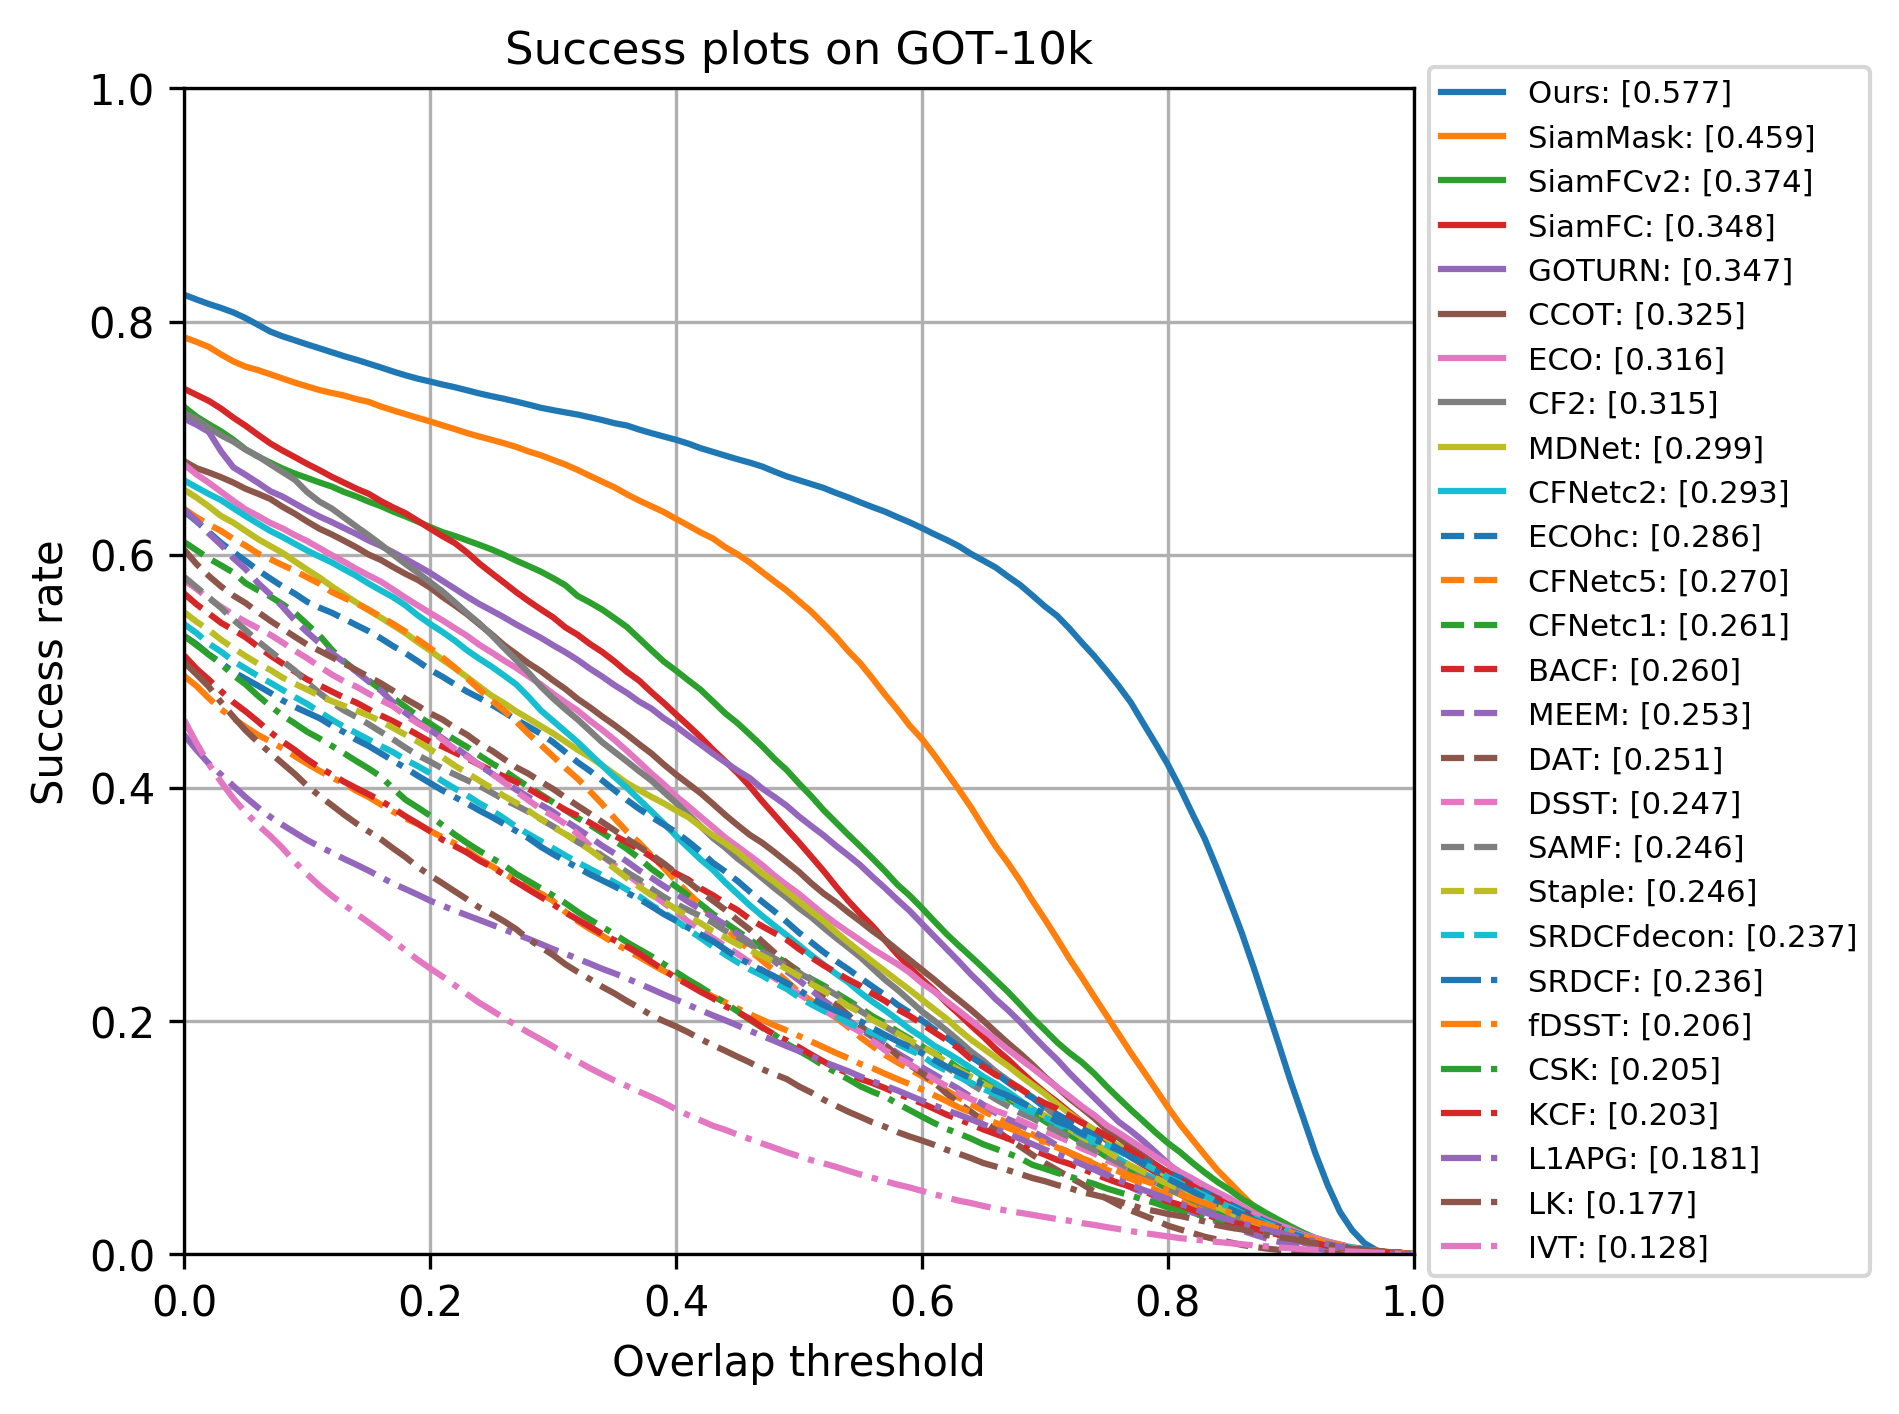
\includegraphics[width=8.6cm]{images/success_plot.png}
    \caption{Overall performance on GOT-10k, ranked by their average overlap (AO) scores.
}
    \label{fig:ao}
\end{figure}
\fi

\subsection{Implementation details}
Our tracking component is trained on the GOT-10k \cite{GOT-10k} training set. It contains more than 10000 video segments of real-world moving objects and over 1.5 million manually labeled bounding boxes, which covers 563 classes of real-world moving objects and 87 classes of motion patterns.
We perform multi-scale training: the target size varies from $64 \times 64$ to $256 \times 256$. The image size remains the same during the tracking progress. The tracking component is trained with stochastic gradient descent (SGD). We use a weight decay of $10^{-4}$ and momentum of 0.9. We train the tracking component for 27k iterations. The learning rate is decreased from $10^{-2}$ to $10^{-4}$.

The motion model is also trained on the GOT-10k training set. The Adam optimizer \cite{kingma2014adam} is adopted for training. The base learning rate is set as $10^{-3}$, and is dropped to $10^{-4}$ and $10^{-5}$ at the 170th and 200th epochs, respectively. The training process is terminated within 210 epochs.

\subsection{Evaluation on GOT-10k Dataset}
In this subsection, we evaluate our method on GOT-10k \cite{GOT-10k} dataset.
The evaluation metric of GOT-10k includes average overlap (AO) and success rate (SR). The AO denotes the average of overlaps between all groundtruth and estimated bounding boxes, while the SR measures the percentage of successfully tracked frames where the overlaps exceed 0.5/0.75.

\textbf{Ablation Studies}
From Table \ref{tabel:ablation} (the $1^{st}$ and $2^{nd}$ row), we see that the AO performance increases by 11.1\% by adding the RoI head. The RPN stage rapidly filters out most background samples, and the RoI head adopts a fixed foreground-to-background ratio to maintain a manageable balance between foreground and background.
From Table \ref{tabel:ablation} (the $2^{nd}$ and $3^{rd}$ row), we see that with the motion model, the AO, the SR$_{0.50}$ and the SR$_{0.75}$ increases by 3.9\%, 5.0\% and 1.7\%, respectively. This is because the proposed motion model can effectively predict the position distribution of the target, effectively avoiding the adverse effects of distractors. 

\textbf{Overall Performance}
We compare our proposed method with 8 trackers including state-of-the-arts, on GOT-10k testing set.
%To reflect the generalization ability, all deep learning based trackers are trained using the GOT-10k training set.
\begin{table}
\centering
\caption{Performance of our algorithm with different components on GOT-10k test set.}
\begin{tabular}{c c c c c}
\bottomrule
ROI head & Motion model & $AO$ & $SR_{0.50}$ & $SR_{0.75}$ \\ 
\hline
          &           & 0.410 & 0.486 & 0.162 \\
\checkmark&           & 0.521 & 0.595 & 0.440 \\
\checkmark&\checkmark & 0.560 & 0.645 & 0.457 \\
\bottomrule
\label{tabel:ablation}
\end{tabular}
\end{table}
\begin{table}
\centering
\caption{Comparing the results of our approach against other approaches over the GOT-10k test set. The trackers are ranked by their average overlap (AO) scores.}
\begin{tabular}{l l l l}
\bottomrule
Method   &  $AO$   &  $SR_{0.50}$ & $SR_{0.75}$  \\
\hline
Ours &  $\textbf{0.560}^\textbf{1}$ & $\textbf{0.645}^\textbf{1}$  & $\textbf{0.457}^\textbf{1}$  \\
SiamMask &  0.459&  0.560 &0.205 \\
SiamFCv2 &  0.374&  0.404 &0.144 \\
SiamFC   &  0.348&  0.353 &0.098 \\
GOTURN	 &  0.347&  0.375 &0.124 \\
CCOT	 &  0.325&  0.328 &0.107 \\
ECO	     &  0.316&  0.309 &0.111 \\
CF2	     &  0.315&  0.297 &0.088 \\
MDNet	 &  0.299&  0.303 &0.099 \\
%CFNetc2	 &  0.293&  0.265 &0.087 \\
%ECOhc	 &  0.286&  0.276 &0.096 \\
\bottomrule
\end{tabular}
\label{table:got}
\end{table}
%The success plot of the evaluated trackers is shown in Fig. \ref{fig:ao}.
Compared to the listed approaches, our approach achieves a superior AO of 0.560 (Table \ref{table:got}).
%CSK is a typical DCF-based tracker, which uses a well-established theory of Circulant matrices to derive closed-form solutions for training and detection with several types of kernels. In contrast, our tracker is based on powerful CNNs. As a result, our tracker significantly outperforms CSK with a relative gain of 173.17\% in terms of AO, which suggests the excellence of the CNN framework as well as the effectiveness of GSTP.
%MDNet learns shared layers and multiple branches of domain-specific layers, where domains correspond to individual training sequences and each branch is responsible for binary classification to identify target in each domain. In contrast, our tracker learns a general similarity map by cross-correlation between the feature representations learned for the target template and the search region. Compared with MDNet, the relative improvement of the AO score is 87.29\%, which suggests that the Siamese architecture and the cross-correlation operation are more suitable for the object tracking task.
%SiamMask is one of state-of-the-art trackers. It is a Siamese tracker and takes advantage of very deep networks to extract features. SiamMask utilizes the region proposal subnetwork to predict the location of the target. 
Compared with SiamMask \cite{Wang2018SiamMask}, our two stage tracker is designed based on the global perception mechanism to reducing cumulative inaccuracies. The motion model suppresses distractors and improves the tracking robustness. As a result, our tracker outperforms SiamMask by relative 22.00\% in terms of AO, which highlights the importance of the proposed tracker and the motion model.

\textbf{Performance Analysis by Attributes} 
\begin{table}
\centering
\caption{Performance on subsets with different attributes collected from GOT-10k validation set.}
\begin{tabular}{|c|c|c|c|c|c|c|}
\hline
\multirow{2}{*}{Att.} &
\multicolumn{2}{c|}{SiamFC} & \multicolumn{2}{c|}{SiamMask} &\multicolumn{2}{c|}{Ours} \\
\cline{2-7} & $AO$ & $SR_{0.5}$ & $AO$ & $SR_{0.5}$ & $AO$ & $SR_{0.5}$ \\
\hline
FM & 0.472 & 0.538 & 0.526 & 0.608 & 0.639 & 0.715 \\
\hline
OC & 0.411 & 0.447 & 0.494 & 0.559 & 0.585 & 0.659 \\
\hline
CU & 0.505 & 0.545 & 0.595 & 0.701 & 0.738 & 0.837 \\
\hline
LO & 0.557 & 0.655 & 0.643 & 0.779 & 0.721 & 0.807 \\
\hline
\end{tabular}
\label{table:attribute}
\end{table}
Every video in GOT-10k training/validation dataset is annotated with multiple attributes including: visible ratios, motion speed, video length and cut by image. To analyze the performance of trackers in various scenarios, we compare our tracker with two state-of-the-art trackers (\textit{i.e.}, SiamFC  \cite{SiamFC} and SiamMask \cite{Wang2018SiamMask}) on GOT-10k validation set. We collect four subset from the validation set according to the attribute annotations: FM (fast motion) subset, OC (occlusion) subset, CU (cut by image) subset, and LO (long video) subset. 
The FM subset includes videos in which the target motion speed is fast.
The OC subset include videos in which the target is occluded frequently.
The CU subset include videos in which the target is cut by the image boundary frequently.
The LO subset includes the longest 40 videos in the validation set.
Table \ref{table:attribute} shows the different performance characteristics of the tracking algorithms.
On the FM subset, our method outperforms SiamMask \cite{Wang2018SiamMask} with a relative gain of 21.48\% in terms of AO. 
%This result suggests that our motion model is capable of modeling challenging motion patterns.
In terms of AO, our algorithm outperforms SiamMask by relative 18.42\% and 24.03\% on OC and CU subset, respectively. 
%This result suggests that our two-stage tracker based on ResNet50 is able to handle the appearance changes caused by heavy occlusion.
On the LO subset, the relative improvement of the AO score is 12.13\% compared with SiamMask. This result shows that the global perception mechanism allows our tracker to reduce the cumulative error when tracking the long videos.

\subsection{Evaluation on UAV20L Dataset}

\begin{figure}[htb]
\begin{minipage}[b]{0.5\linewidth}
  \centering
  \centerline{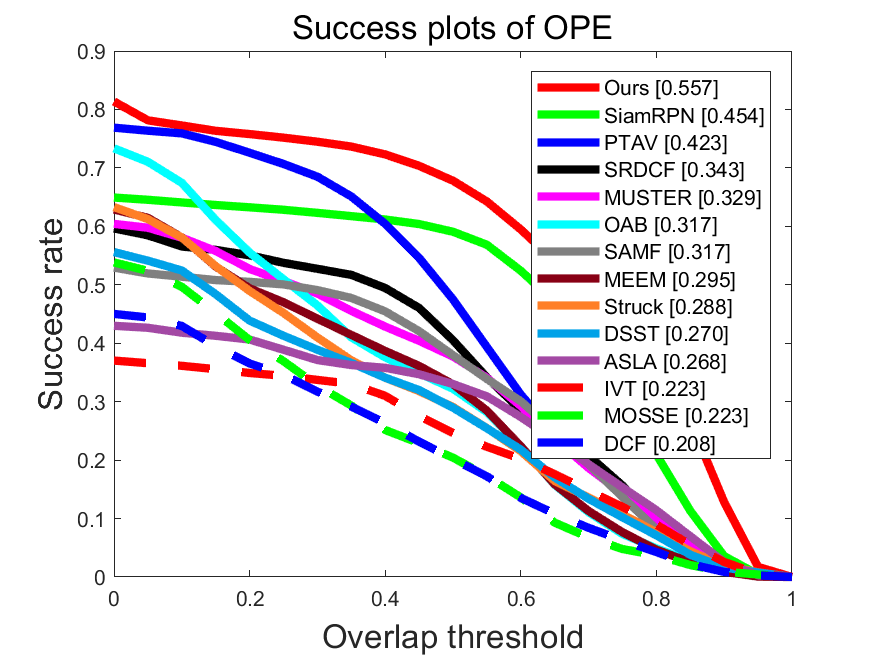
\includegraphics[width=1.0\textwidth]{Img/globally/UAV20L/quality_plot_overlap_OPE_AUC.png}}
\end{minipage}
\hfill
\begin{minipage}[b]{0.5\linewidth}
  \centering
  \centerline{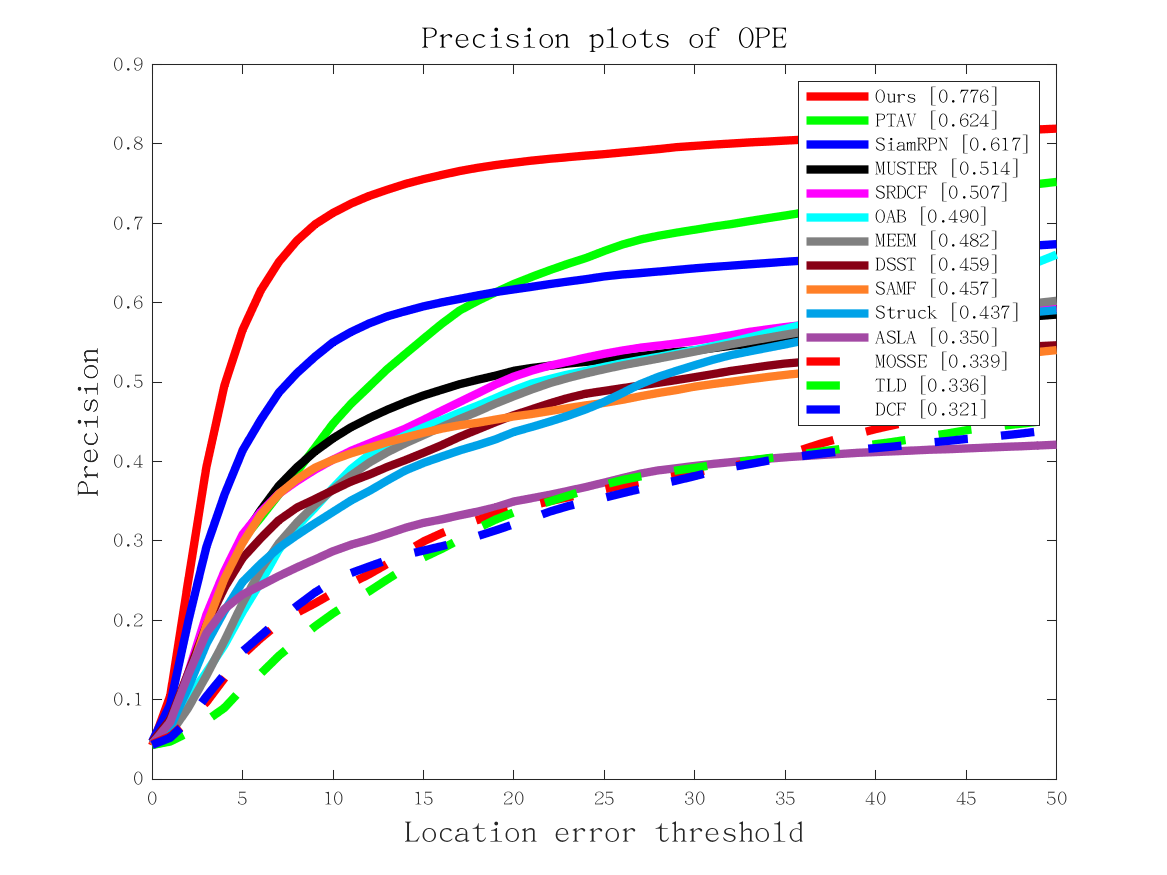
\includegraphics[width=1.0\textwidth]{Img/globally/UAV20L/quality_plot_error_OPE_threshold.png}}
\end{minipage}
%
\caption{Success and precision plots on UAV20L dataset.}
\label{fig:uav20l}
%
\end{figure}

\iffalse
\begin{figure}[t]
\begin{center}
\subfigure[]{
	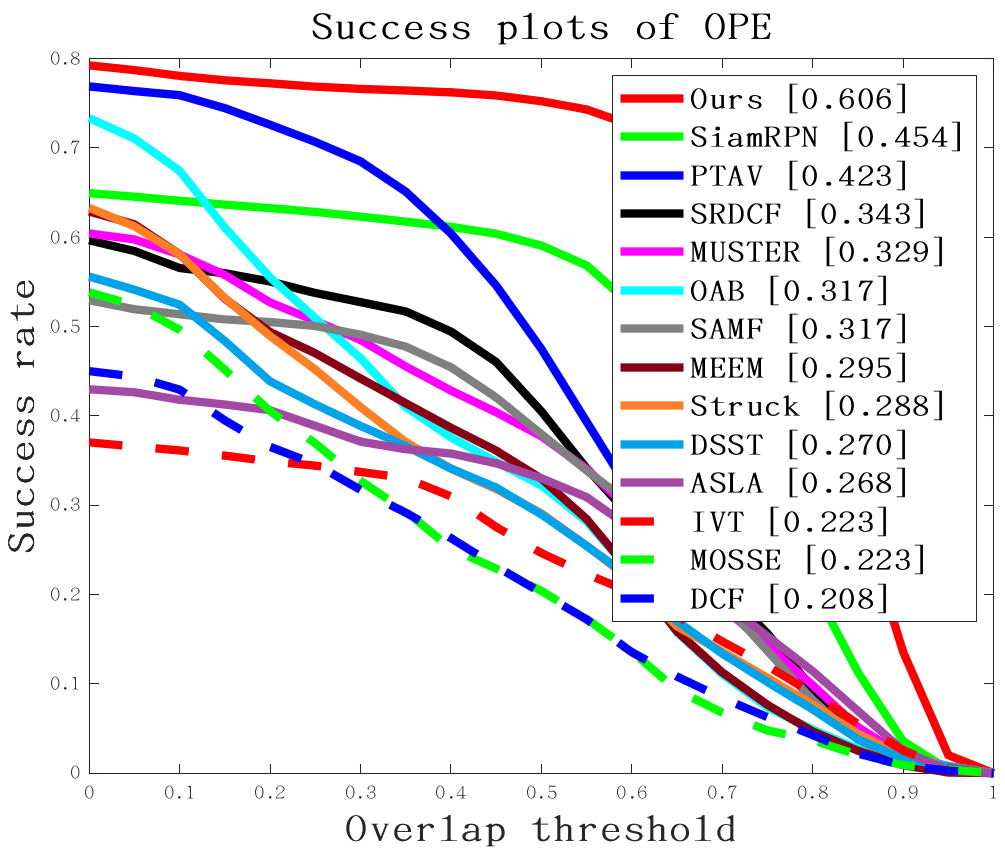
\includegraphics[width=0.47\linewidth]
	{images/UAV20L/quality_plot_overlap_OPE_AUC.png}
}
\subfigure[]{
	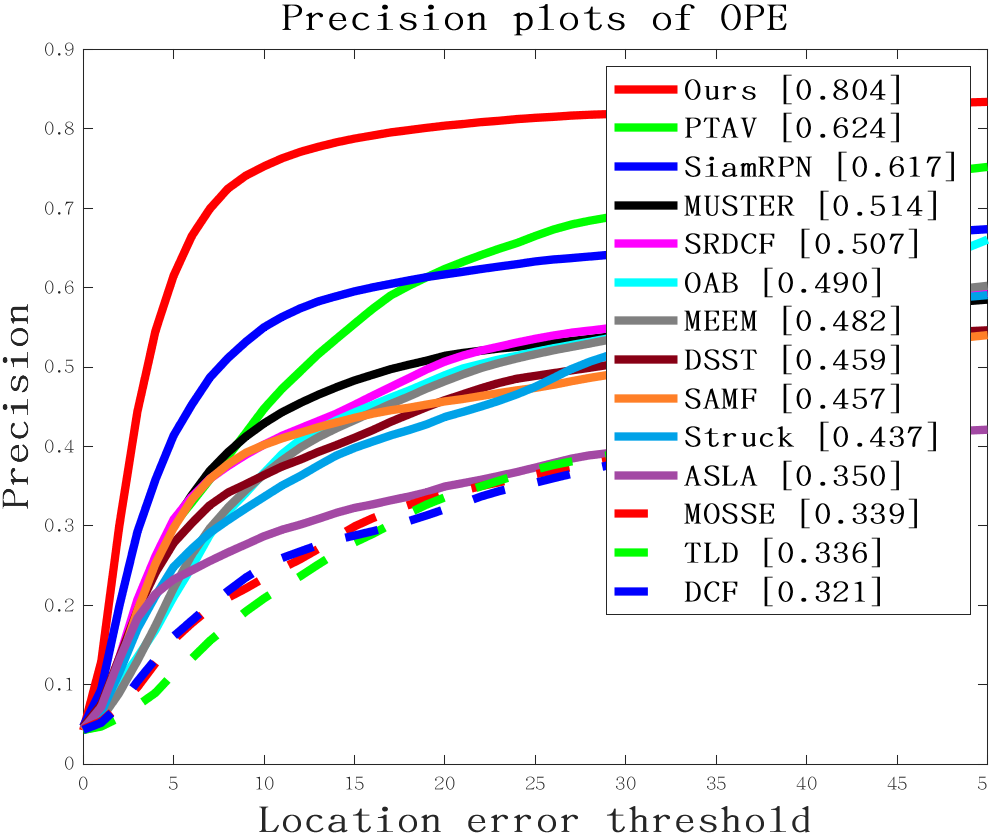
\includegraphics[width=0.47\linewidth]
	{images/UAV20L/quality_plot_error_OPE_threshold.png}
}
\end{center}
   \caption{Success and precision plots on UAV20L dataset.}
\label{fig:uav20l}
\end{figure}

\begin{figure*}
\begin{center}
\subfigure[]{
	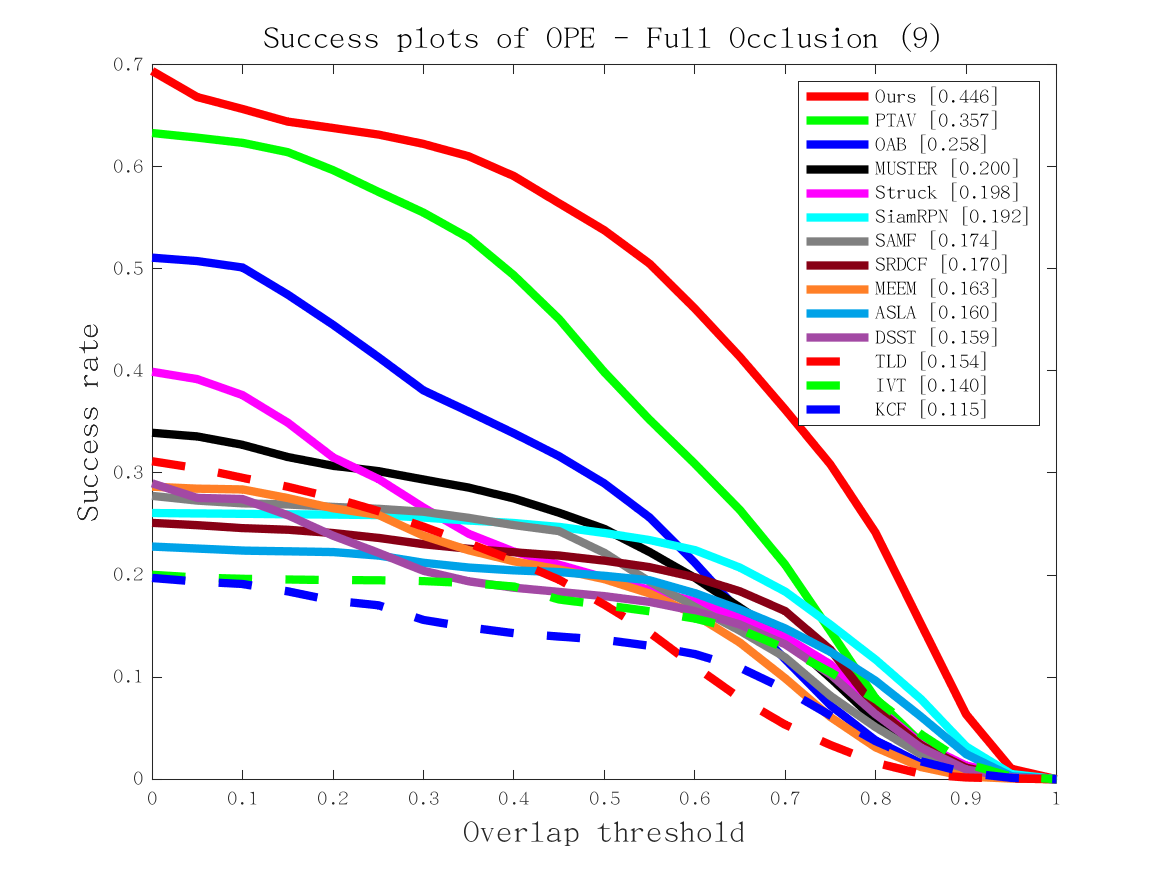
\includegraphics[width=0.234\linewidth]
	{images/UAV20L/FOC_overlap_OPE_AUC.png}
}
\subfigure[]{
	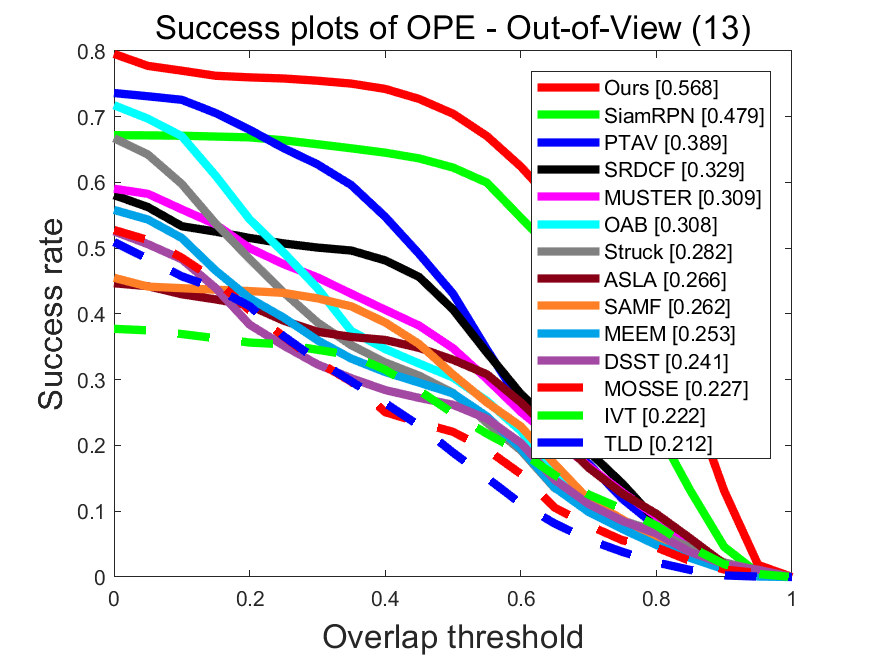
\includegraphics[width=0.234\linewidth]
	{images/UAV20L/OV_overlap_OPE_AUC.png}
}
\subfigure[]{
	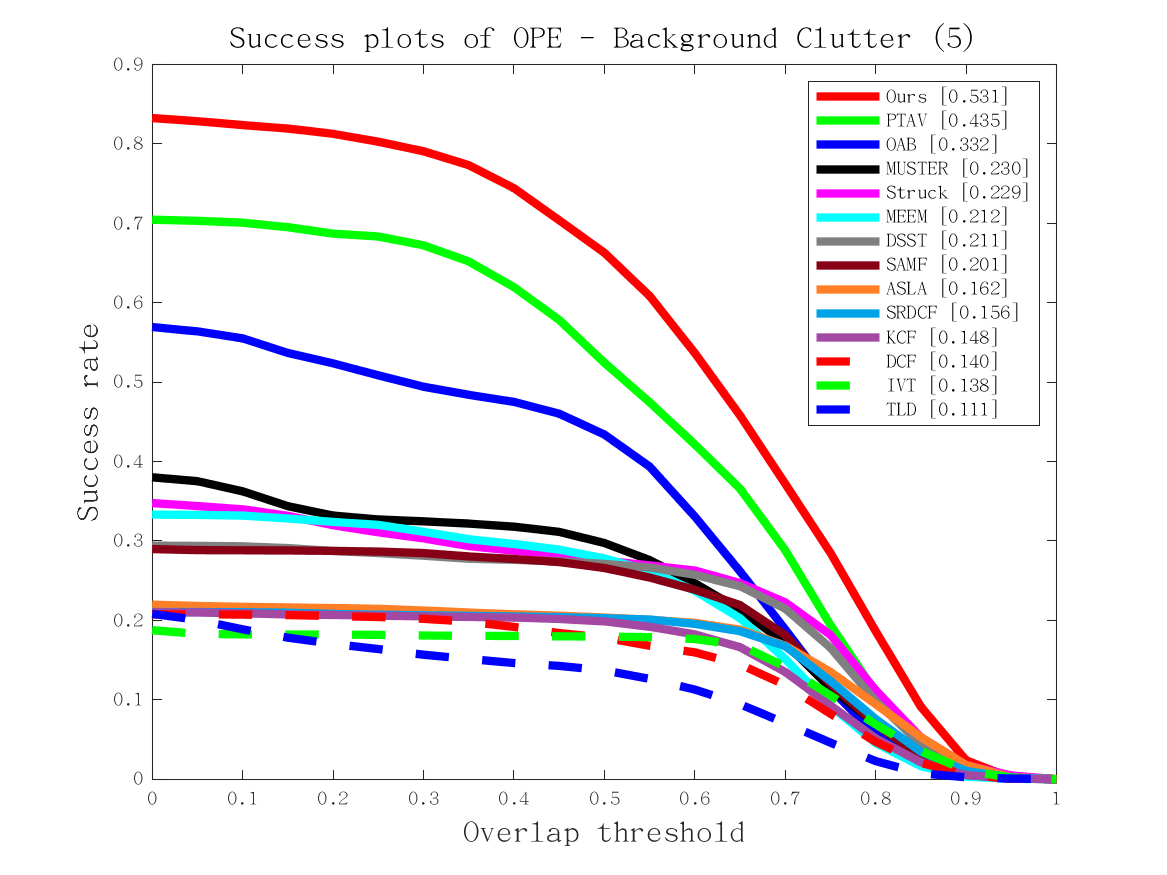
\includegraphics[width=0.234\linewidth]
	{images/UAV20L/BC_overlap_OPE_AUC.png}
}
\subfigure[]{
	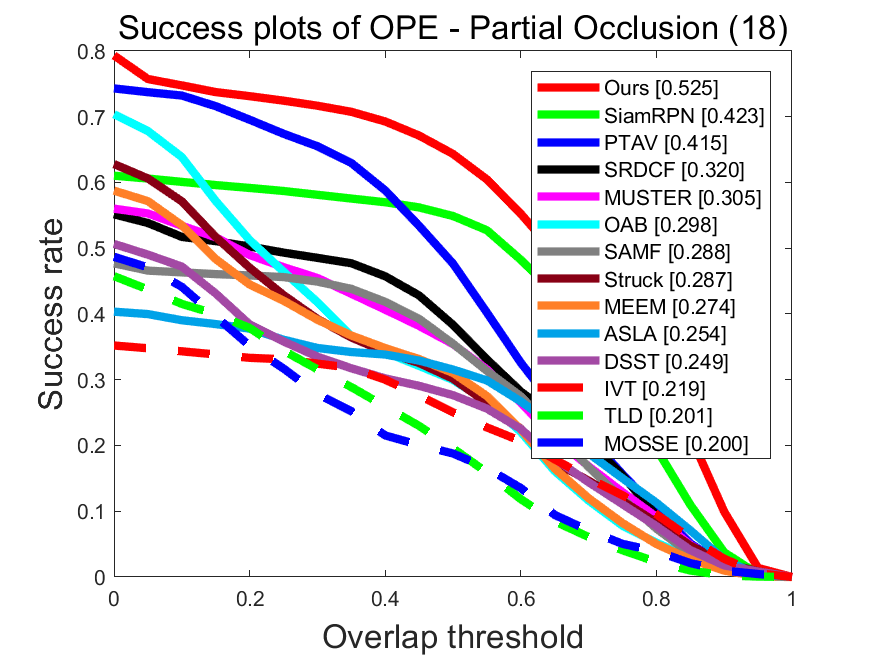
\includegraphics[width=0.234\linewidth]
	{images/UAV20L/POC_overlap_OPE_AUC.png}
}
\subfigure[]{
	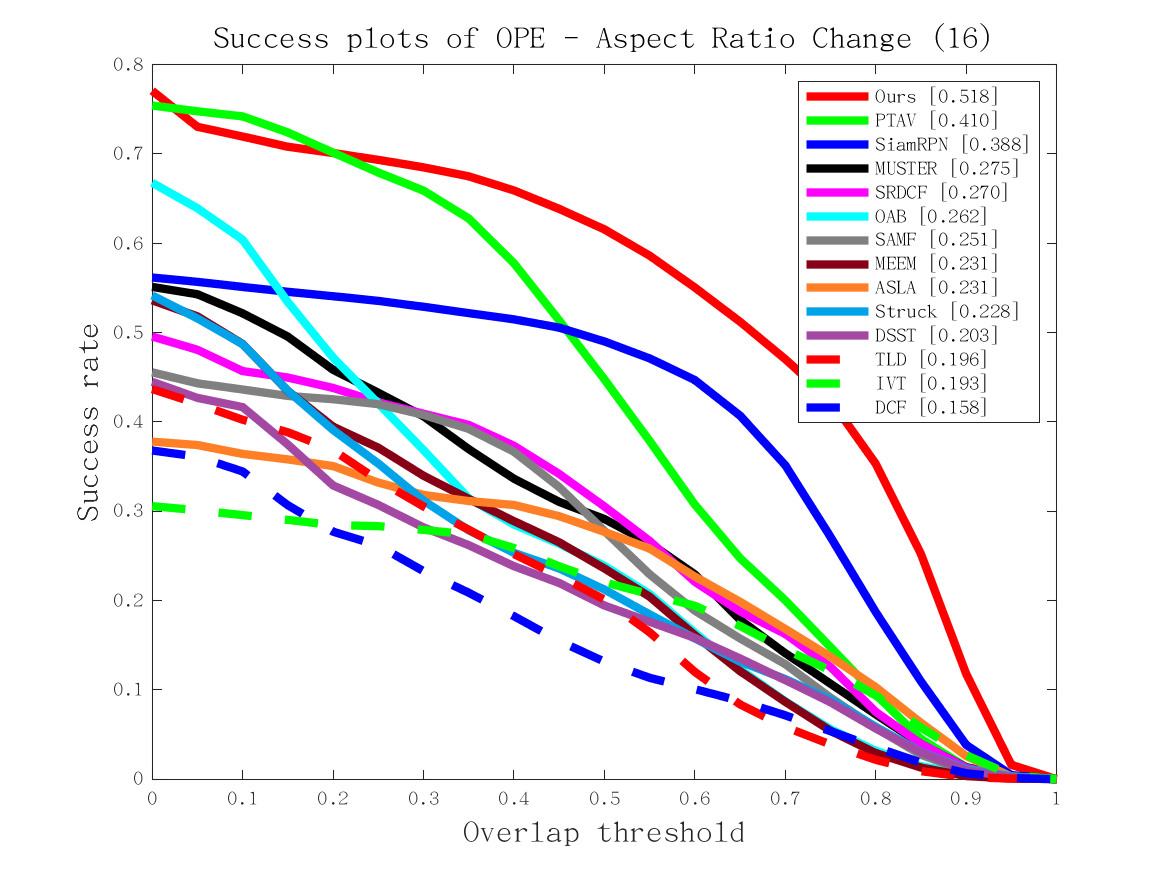
\includegraphics[width=0.234\linewidth]
	{images/UAV20L/ARC_overlap_OPE_AUC.png}
}
\subfigure[]{
	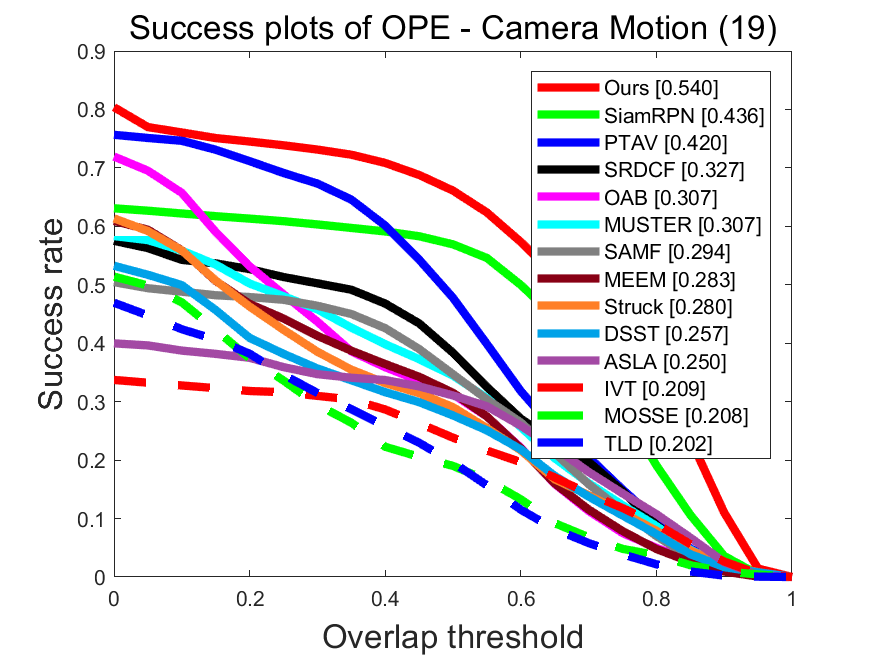
\includegraphics[width=0.234\linewidth]
	{images/UAV20L/CM_overlap_OPE_AUC.png}
}
\subfigure[]{
	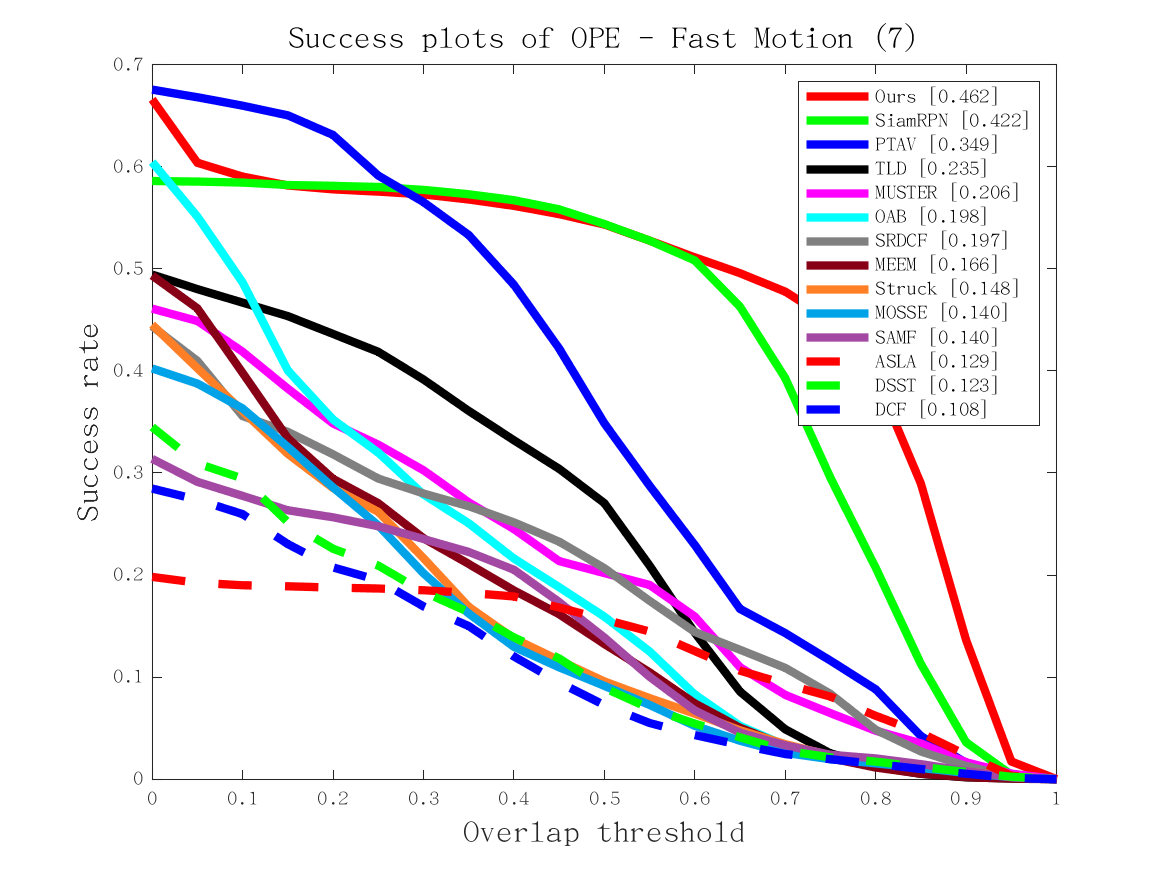
\includegraphics[width=0.234\linewidth]
	{images/UAV20L/FM_overlap_OPE_AUC.png}
}
\subfigure[]{
	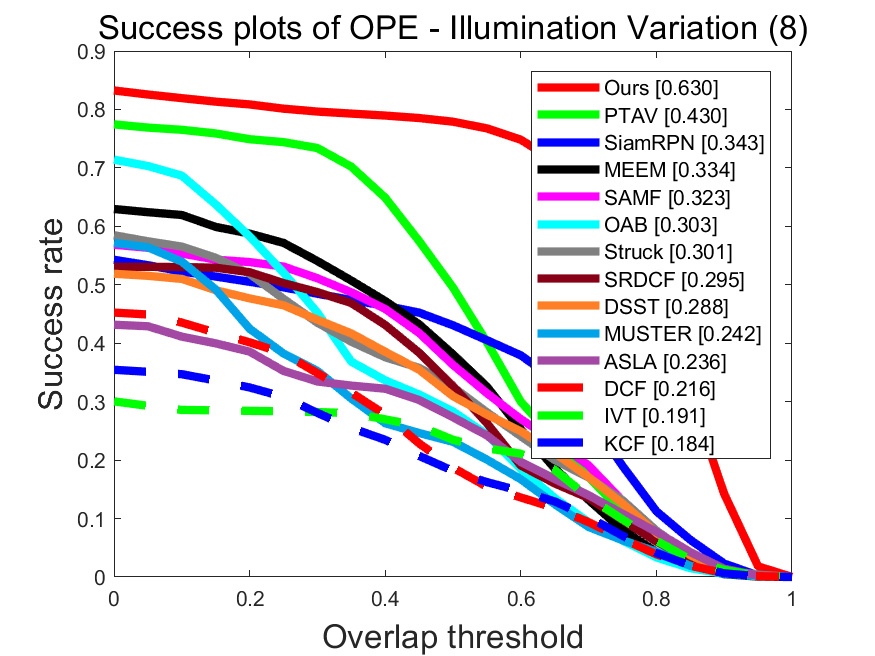
\includegraphics[width=0.234\linewidth]
	{images/UAV20L/IV_overlap_OPE_AUC.png}
}
\subfigure[]{
	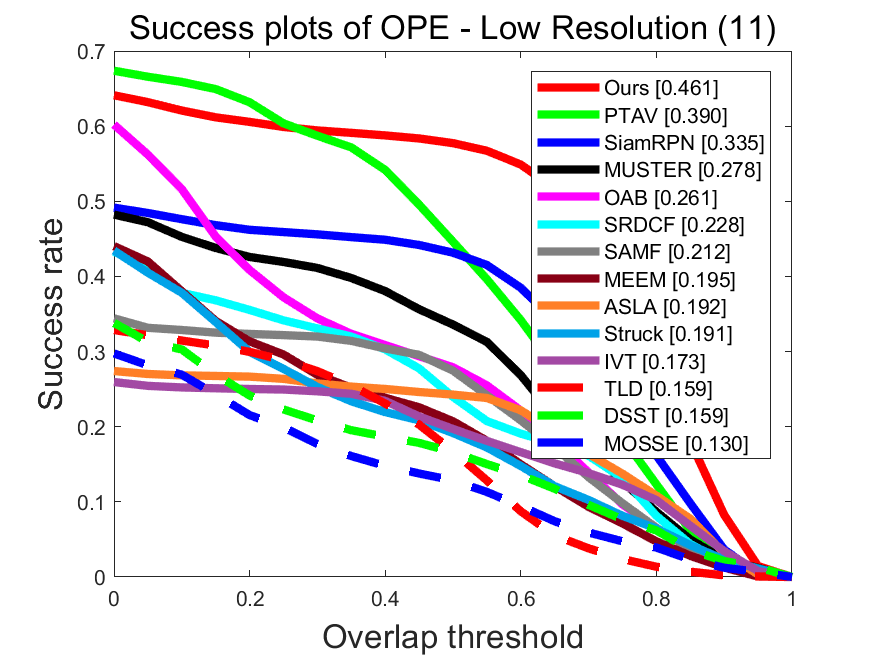
\includegraphics[width=0.234\linewidth]
	{images/UAV20L/LR_overlap_OPE_AUC.png}
}
\subfigure[]{
	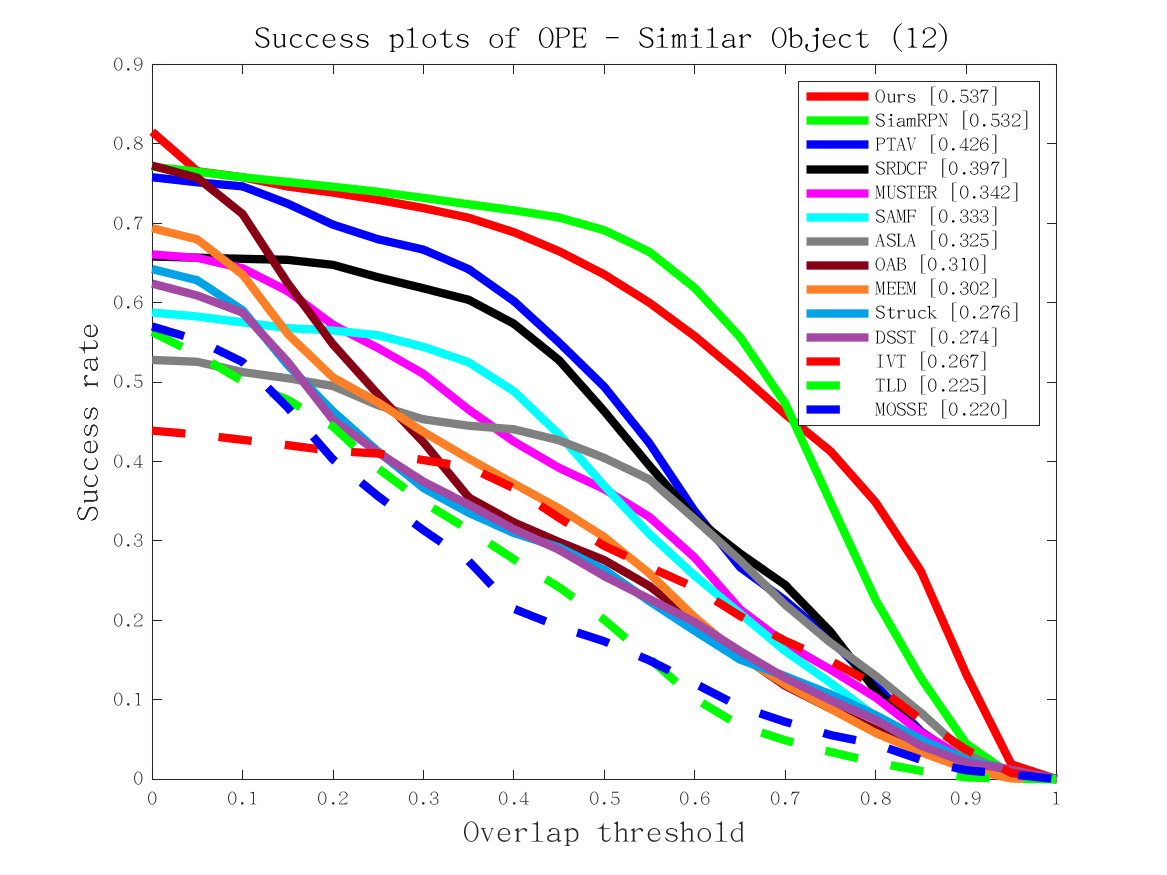
\includegraphics[width=0.234\linewidth]
	{images/UAV20L/SOB_overlap_OPE_AUC.png}
}
\subfigure[]{
	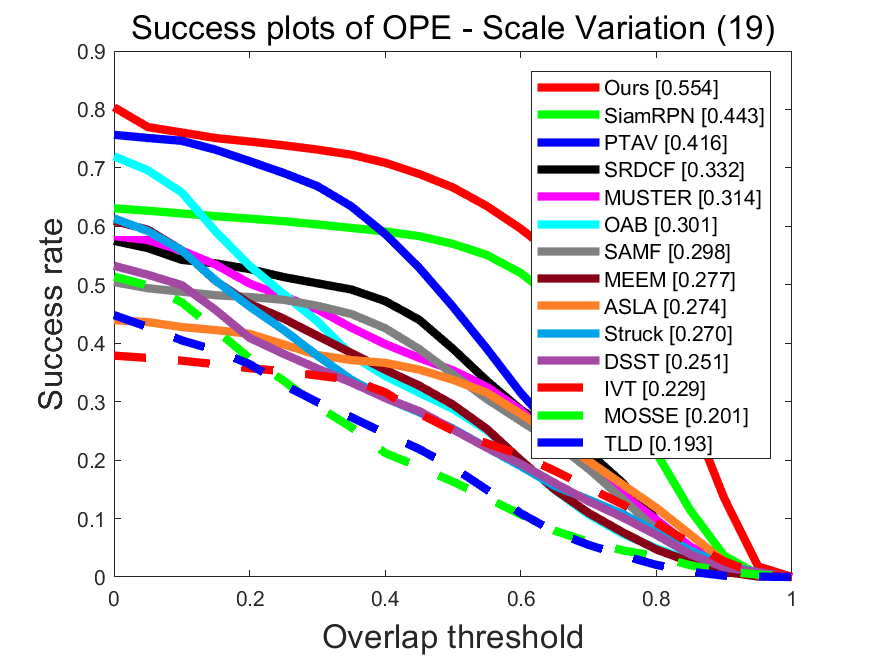
\includegraphics[width=0.234\linewidth]
	{images/UAV20L/SV_overlap_OPE_AUC.png}
}
\subfigure[]{
	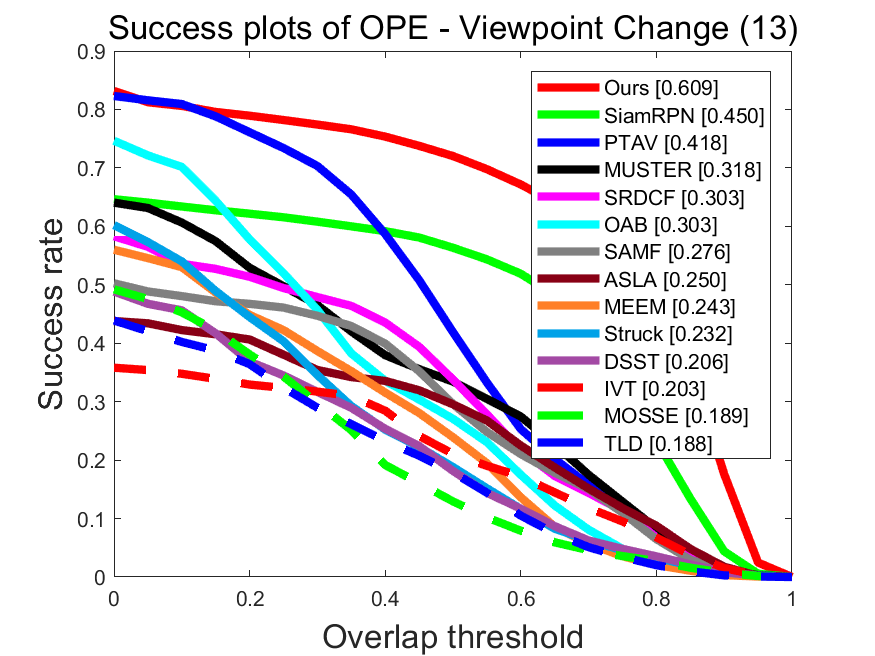
\includegraphics[width=0.234\linewidth]
	{images/UAV20L/VC_overlap_OPE_AUC.png}
}
\end{center}
   \caption{Success plots with attributes on UAV20L. Best viewed on color display.}
\label{fig:uav20l_attr}
\end{figure*}
\fi

UAV20L \cite{mueller2016benchmark} is an aerial video dataset captured from a low-altitude aerial perspective. Designed for long-term tracking, the UAV20L database has 20 videos with an average length of 2934 frames. 
Following the evaluation method of OTB50 \cite{OTB}, we use precision and success to evaluate the performance of  trackers on the UAV20L dataset. Precision refers to the distance from the center point of the predicted bounding box to the center point of the ground truth bounding box. Success refers to the intersection over union (IOU) of the predicted bounding box and the ground truth bounding box. In Fig. \ref{fig:uav20l}, the performance comparison of different trackers is visualized by precision plot and success plot.

The proposed method is compared against 13 recent trackers. Fig. \ref{fig:uav20l} clearly shows that our algorithm outperforms all other trackers in terms of success and precision scores. Specifically, in the success plot, our tracker obtains a AUC score of 0.557. Compared with the state-of-art method PTAV \cite{fan2018parallel} and SiamRPN \cite{SiamRPN}, the proposed tracker outperforms these trackers by relative 31.7\% and 22.7\%. In the precision plot, the proposed algorithm obtains a score of 0.776. Compared with SiamRPN \cite{SiamRPN} and PTAV \cite{fan2018parallel}, the proposed tracker outperforms these trackers by relative 25.8\% and 24.4\%. 

\iffalse
In order to perform a more in-depth and detailed analysis of the performance of the trackers, we also report the results on challenging attributes in UAV20L. Fig. \ref{fig:uav20l_attr} lists the success plots of 14 different methods on 12 attributes: ARC (Aspect Ratio Change), BC (Background Clutter), CM (Camera Motion), FM (Fast Motion), FOC (Full Occlusion), IV (Illumination Variation), LR (LR Low Resolution), OV (Out-of-View), POC (Partial Occlusion), SOB (Similar Object), SV (Scale Variation) and VC (Viewpoint Change). We can observe that the AUC of the proposed algorithm perform better than other methods on most challenging attributes, which means our method is more robust than other approaches on various difficult situations.
\fi

\section{CONCLUSION}
\label{sec:conclusion}

In this paper, we propose a novel tracking architecture including the tracking component and the data-driven motion model. The global perception mechanism allows the tracking component to reduce the cumulative error during the tracking process. The tracking component uses a very deep network for two-stage tracking, which makes the tracker more discriminative. The motion model is trained end-to-end and is capable of learning the motion patterns of targets from large-scale trajectory datasets. Through the collaborative work of the tracking component and the motion model, the proposed method performs favorably against state-of-the-art trackers.